\documentclass[9pt]{article}

\usepackage[T1]{fontenc}
\usepackage[polish]{babel}
\usepackage{geometry}
\usepackage{graphicx}
\usepackage{algorithm}
\usepackage{algpseudocode}
\usepackage{amsmath}

\title{
    \huge \textbf{Projekt 2 - Eliminacja Gaussa i LU faktoryzacja}\\~\\
    \LARGE Temat - Zaimplementować dla macierzy o rozmiarze = (
    miesiąc urodzenia + dzień urodzenia)
    
    1) Algorytm eliminacji Gaussa bez pivotingu generujący jedynki na przekątnej (slajd 14)
    
    2) Algorytm eliminacji Gaussa z pivotingiem (slajd 26)
    
    3) Algorytm LU faktoryzacji bez pivotingu (slajd 33)
    
    4) Algorytm LU faktoryzacji z pivotingiem (slajd 36)
}
\author{Bartłomiej Jamiołkowski}
\date{}

\begin{document}
\maketitle

W projekcie macierz ma rozmiar N = 15, ponieważ jest to suma mojego dnia i miesiąca urodzenia, czyli 10.05.

\section{Algorytm eliminacji Gaussa bez pivotingu generujący jedynki na
przekątnej}

\subsection{Pseudokod}

\begin{algorithm}
\caption{Gaussian Elimination without Pivoting}
\begin{algorithmic}[1]
\Require $A$ - a square matrix $n \times n$
\Require $b$ - a column vector $n \times 1$
\Ensure $x$ - a column vector $n \times 1$ representing the solution to the system of equations $Ax = b$
\For{$i = 0$ \textbf{to} $n-1$}
    \For{$j = 0$ \textbf{to} $n-1$}
        \If{$j == i$}
            \State $b[i] \gets b[i] / A[i, i]$
            \State $A[i, :] \gets A[i, :] / A[i, i]$
        \ElsIf{$j > i$}
            \State $b[j] \gets b[j] - b[i] \times A[j, i]$
            \State $A[j, :] \gets A[j, :] - A[i, :] \times A[j, i]$
        \EndIf
    \EndFor
\EndFor
\State $x \gets \text{SolveUpperTriangular}(A, b)$ \Comment{Solve system of equations with upper triangular matrix $A$}
\State \textbf{return} $x$
\end{algorithmic}
\end{algorithm}
\newpage

Działanie programu można wyjaśnić następująco:

\begin{enumerate}
    \item Funkcja przyjmuje dwie argumenty: macierz kwadratową $A$ oraz wektor kolumnowy $b$.
    
    \item Pętla zewnętrzna \texttt{for} $i$ \texttt{in} \texttt{range}$(A.shape[0])$ iteruje po wierszach macierzy $A$.
    
    \item Wewnętrzna pętla \texttt{for} $j$ \texttt{in} \texttt{range}$(A.shape[1])$ iteruje po kolumnach macierzy $A$.
    
    \item Warunek \texttt{if} $j == i$ sprawdza, czy aktualna kolumna odpowiada obecnie przetwarzanemu wierszowi. Innymi słowy sprawdza czy element macierzy jest na jej przekątnej. Jeśli tak, to wykonują się następujące czynności:
    \begin{itemize}
        \item Element $b[i]$ dzielony jest przez odpowiadający element na przekątnej macierzy $A$ (element diagonalny).
        \item Cały wiersz $A[j, :]$ dzielony jest przez element przekątnej $A[i, i]$. Dzięki temu element na przekatnej staje się równy $1$.
    \end{itemize}
    
    \item Warunek \texttt{elif} $j > i$ odnosi się do kolumn poza główną przekątną macierzy $A$. Dla tych kolumn wykonują się następujące czynności:
    \begin{itemize}
        \item Elementy wektora $b$ są aktualizowane przez odjęcie iloczynu $b[i]$ i elementu $A[j, i]$.
        \item Wiersze macierzy $A$ są aktualizowane poprzez odjęcie iloczynu wiersza $A[i, :]$ i elementu $A[j, i]$. Dzieje się to w celu wyeliminowania niezerowych wartości pod główną przekątną macierzy.
    \end{itemize}
    
    \item Proces ten kontynuuje się dla kolejnych wierszy i kolumn, aż do zakończenia przetwarzania całej macierzy $A$.
    
    \item Na koniec działania funkcji zwracana jest przekształcona macierz $A$ oraz zaktualizowany wektor $b$, które zawierają rozwiązania układu równań po eliminacji Gaussa w {x}.
\end{enumerate}

\subsection{Kod algorytmu w języku Python}

\begin{figure}[h]
  \centering
  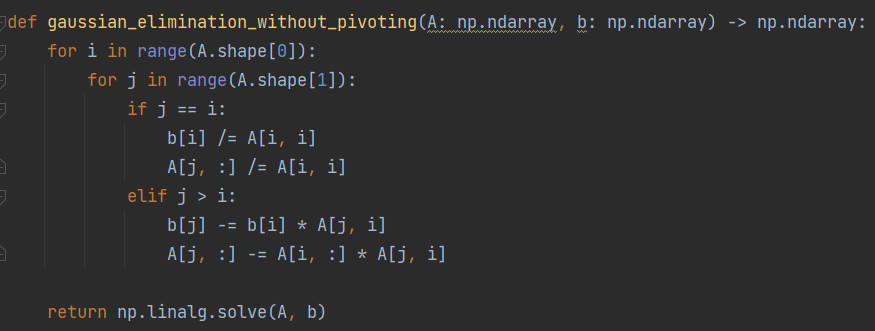
\includegraphics[width=0.8\textwidth]{gaussian_elimination_without_pivoting.jpg}
  \caption{Kod algorytmu eliminacji Gaussa generujący 1 na przekątnej}
\end{figure}

\subsection{Test dla macierzy gęstej o losowych wartościach (porównanie z MATLAB)}

Sprawdzenie czy algorytm generuje jedynki na przekątnej.

\begin{figure}[h]
  \centering
  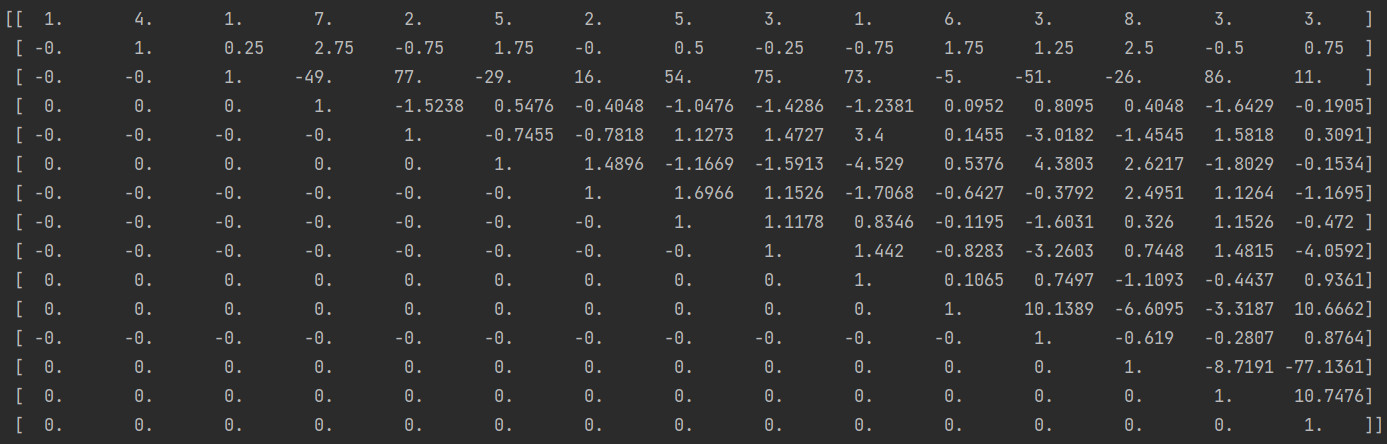
\includegraphics[width=0.9\textwidth]{ones_on_diagonal.jpg}
  \caption{Przekształcona macierz górna trójkątna A z 1 na przekątnej}
\end{figure}

Losowanie macierzy gęstej A z wartościami losowymi.

\begin{figure}[h]
  \centering
  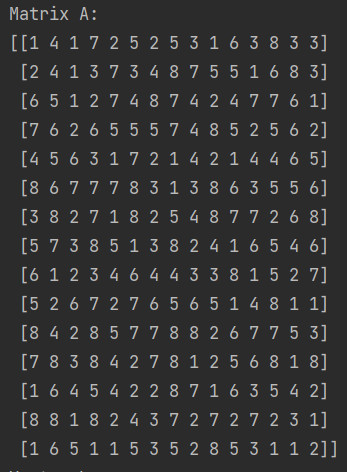
\includegraphics[width=0.6\textwidth]{matrix_A_1.jpg}
  \caption{Macierz gęsta A}
\end{figure}
\newpage

Losowanie wektora b prawej strony z wartościami losowymi.

\begin{figure}[h]
  \centering
  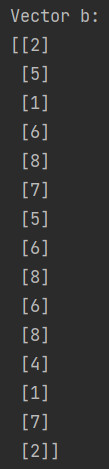
\includegraphics[width=0.1\textwidth]{vector_B_1.jpg}
  \caption{Wektor prawej strony b}
\end{figure}
\newpage

Rozwiązanie układu równań moim programem.

\begin{figure}[h]
  \centering
  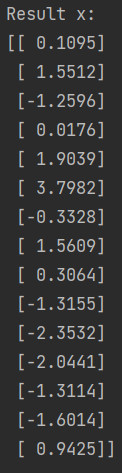
\includegraphics[width=0.1\textwidth]{result_x_1.jpg}
  \caption{Rozwiązanie układu równań x}
\end{figure}
\newpage

Rozwiązanie układu równań programem MATLAB.

\begin{figure}[h]
  \centering
  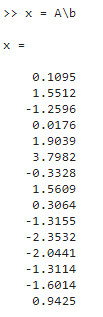
\includegraphics[width=0.2\textwidth]{result_x_matlab_1.jpg}
  \caption{Rozwiązanie układu równań x w MATLAB}
\end{figure}

Porównanie wyników mojego programu i MATLAB norm(x1-x2,2).

\begin{figure}[h]
  \centering
  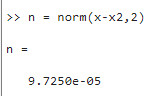
\includegraphics[width=0.2\textwidth]{results_x_comparison_1.jpg}
  \caption{Wynik rnorm(x1 - x2, 2) x w MATLAB}
\end{figure}

Na podstawie wydrukowanych przez programy wyników można zauważyć, że w tym przypadku są one takie same. Potwierdza to wynik 9.7250e-05 w MATLAB, który wskazuje, że różnice między poszczególnymi wynikami w wektorach x1 i x2 są bardzo małe.

\section{Algorytm eliminacji Gaussa z pivotingiem}

\subsection{Pseudokod}

\begin{algorithm}
\caption{Gaussian Elimination with Pivoting}
\begin{algorithmic}[1]
\Require $A$ is a square matrix
\Require $b$ is a vector
\Ensure Solution vector $x$ of the linear system $Ax = b$
    \For{$i \gets 0$ \textbf{to} $A.\text{shape}[0] - 1$}
        \State $A[\{i, -1\}] \gets A[\{-1, i\}]$
        \State $b[i], b[-1] \gets b[-1], b[i]$
        \For{$j \gets 0$ \textbf{to} $A.\text{shape}[1] - 1$}
            \If{$j > i$}
                \State $b[j] \gets b[j] - \frac{b[i] \times A[j, i]}{A[i, i]}$
                \State $A[j, :] \gets A[j, :] - \frac{A[i, :] \times A[j, i]}{A[i, i]}$
            \EndIf
        \EndFor
    \EndFor
    \State \textbf{return} $\text{solve\_linear\_equations}(A, b)$
\end{algorithmic}
\end{algorithm}
\newpage

Działanie programu można wyjaśnić następująco:

\begin{enumerate}
    \item Funkcja \texttt{gaussian\_elimination\_with\_pivoting} wykonuje eliminację Gaussa z częściowym wyborem elementu podstawowego w celu rozwiązania układu równań liniowych.
    \item Przyjmuje dwa argumenty: \texttt{A}, tablicę numpy reprezentującą macierz współczynników równań liniowych, oraz \texttt{b}, tablicę numpy reprezentującą wektor stałych.
    \item Funkcja najpierw iteruje po wierszach macierzy współczynników \texttt{A}.
    \item W każdej iteracji zamienia bieżący wiersz z ostatnim wierszem w celu przeprowadzenia częściowego wyboru elementu podstawowego. Pomaga to uniknąć dzielenia przez zero i problemów z niestabilnością numeryczną.
    \item Zmienia również odpowiednie elementy wektora stałego \texttt{b} zgodnie z zamianą.
    \item Następnie przechodzi do eliminacji współczynników poniżej diagonalnej dla każdej kolumny, zapewniając, że macierz staje się górnotrójkątna.
    \item Podczas eliminacji aktualizuje zarówno macierz współczynników \texttt{A}, jak i wektor stały \texttt{b}.
    \item Po zakończeniu procesu eliminacji funkcja używa funkcji \texttt{linalg.solve} z biblioteki numpy do rozwiązania układu równań reprezentowanego przez zmodyfikowane \texttt{A} i \texttt{b}.
    \item Na koniec zwraca wektor rozwiązania \(x\) uzyskany z procesu rozwiązywania.
\end{enumerate}

\subsection{Kod algorytmu w języku Python}

\begin{figure}[h]
  \centering
  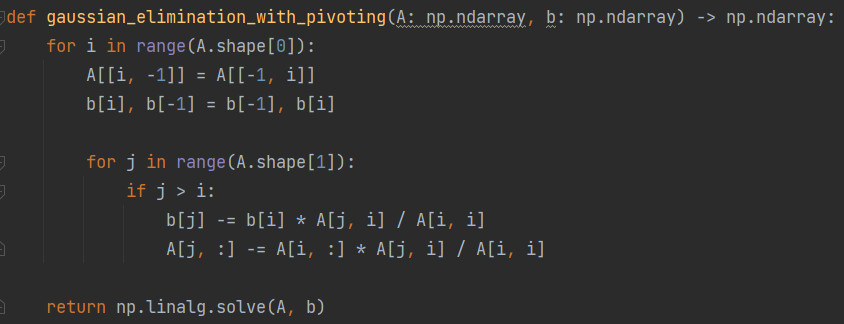
\includegraphics[width=0.9\textwidth]{gaussian_elimination_with_pivoting.jpg}
  \caption{Kod algorytmu eliminacji Gaussa z pivotingiem}
\end{figure}
\newpage

\subsection{Test dla macierzy gęstej o losowych wartościach (porównanie z MATLAB)}

Sprawdzenie czy algorytm generuje rózne wartości na przekątnej.

\begin{figure}[h]
  \centering
  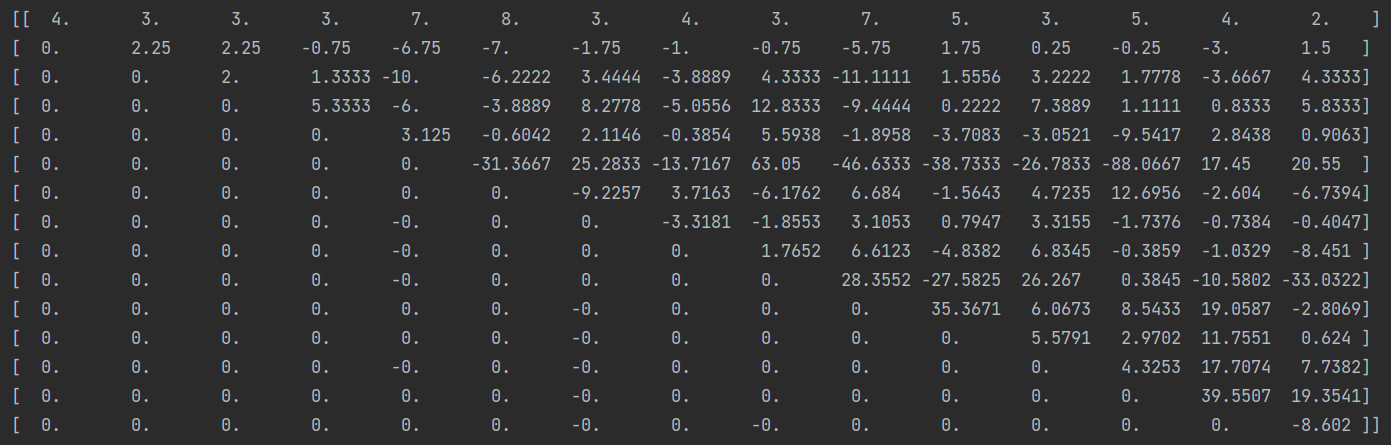
\includegraphics[width=0.9\textwidth]{values_on_diagonal.jpg}
  \caption{Przekształcona macierz górna trójkątna A}
\end{figure}

Losowanie macierzy gęstej A z wartościami losowymi.

\begin{figure}[h]
  \centering
  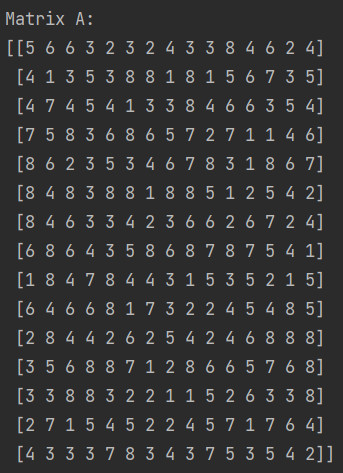
\includegraphics[width=0.6\textwidth]{matrix_A_2.jpg}
  \caption{Macierz gęsta A}
\end{figure}
\newpage

Losowanie wektora b prawej strony z wartościami losowymi.

\begin{figure}[h]
  \centering
  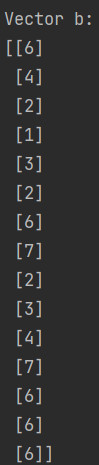
\includegraphics[width=0.1\textwidth]{vector_B_2.jpg}
  \caption{Wektor prawej strony b}
\end{figure}
\newpage

Rozwiązanie układu równań moim programem.

\begin{figure}[h]
  \centering
  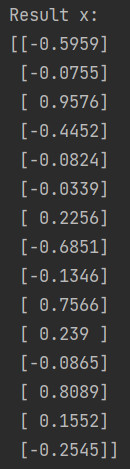
\includegraphics[width=0.1\textwidth]{result_x_2.jpg}
  \caption{Rozwiązanie układu równań x}
\end{figure}
\newpage

Rozwiązanie układu równań programem MATLAB.

\begin{figure}[h]
  \centering
  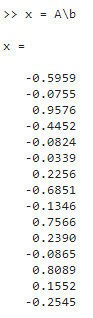
\includegraphics[width=0.2\textwidth]{result_x_matlab_2.jpg}
  \caption{Rozwiązanie układu równań x w MATLAB}
\end{figure}
\newpage

Porównanie wyników mojego programu i MATLAB norm(x1-x2,2).

\begin{figure}[h]
  \centering
  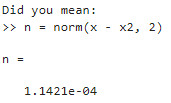
\includegraphics[width=0.2\textwidth]{results_x_comparison_2.jpg}
  \caption{Wynik norm(x1 - x2, 2) x w MATLAB}
\end{figure}

Na podstawie wydrukowanych przez programy wyników można zauważyć, że w tym przypadku są one takie same. Potwierdza to wynik 1.1421e-04 w MATLAB, który wskazuje, że różnice między poszczególnymi wynikami w wektorach x1 i x2 są bardzo małe.

\section{Algorytm LU faktoryzacji bez pivotingu}

\subsection{Pseudokod}

\begin{algorithm}
    \caption{LU factorization without pivoting}
    \begin{algorithmic}[1]
        \Require $A$ is a square matrix
        \Require $b$ is a vector
        \Ensure Solution vector $x$ of the linear system $Ax = b$
        \State $L \gets \text{identity\_matrix}(A.\text{shape}[0])$
        \For{$i$ \textbf{in} $\text{range}(A.\text{shape}[0])$}
            \For{$j$ \textbf{in} $\text{range}(A.\text{shape}[1])$}
                \If{$j > i$}
                    \State $L[j, i] \gets A[j, i] / A[i, i]$
                    \State $B[j] \gets B[j] - B[i] \times A[j, i] / A[i, i]$
                    \State $A[j, :] \gets A[j, :] - A[i, :] \times A[j, i] / A[i, i]$
                \EndIf
            \EndFor
        \EndFor
        \State $U \gets A.\text{copy}()$
        \State \textbf{return} $L, U$
    \end{algorithmic}
\end{algorithm}

Działanie programu można wyjaśnić następująco:

\begin{enumerate}
    \item Funkcja \texttt{lu\_factorization\_without\_pivoting} przeprowadza faktoryzację LU bez wyboru elementu podstawowego dla danej macierzy kwadratowej A.
    \item Przyjmuje dwa argumenty: \texttt{A}, tablicę numpy reprezentującą macierz współczynników, oraz \texttt{B}, tablicę numpy reprezentującą wektor stałych.
    \item Inicjuje dolnotrójkątną macierz \texttt{L} jako macierz identycznościową tej samej wielkości co \texttt{A}.
    \item Funkcja iteruje po wierszach i kolumnach macierzy \texttt{A}.
    \item Dla każdego elementu \texttt{A[j, i]} w \texttt{A}, gdzie \texttt{j} jest większe niż \texttt{i}, oblicza odpowiednią wartość w dolnotrójkątnej macierzy \texttt{L} używając wzoru \texttt{L[j, i] = A[j, i] / A[i, i]}.
    \item Aktualizuje elementy wektora stałych \texttt{B}, odejmując \texttt{B[i] * A[j, i] / A[i, i]} od \texttt{B[j]}.
    \item Przeprowadza eliminację Gaussa na wierszach \texttt{A} poniżej diagonali, aktualizując odpowiednio \texttt{A} i \texttt{B}.
    \item Po zakończeniu procesu eliminacji funkcja tworzy górnotrójkątną macierz \texttt{U} poprzez skopiowanie \texttt{A}.
    \item Na koniec zwraca krotkę \texttt{(L, U)} zawierającą dolnotrójkątną macierz \texttt{L} i górnotrójkątną macierz \texttt{U}.
\end{enumerate}

\subsection{Kod algorytmu w języku Python}

\begin{figure}[h]
  \centering
  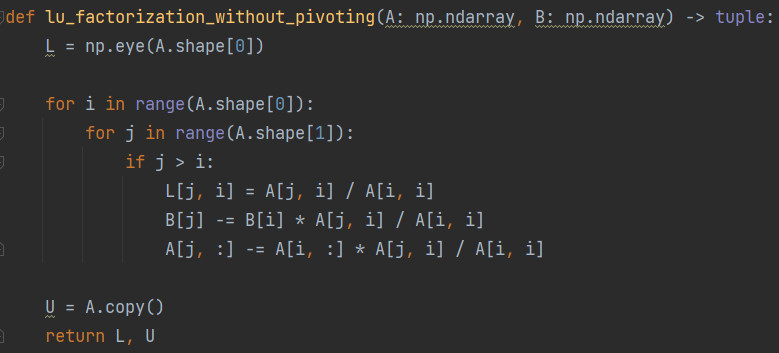
\includegraphics[width=0.9\textwidth]{lu_factorization_without_pivoting.jpg}
  \caption{Kod algorytmu LU faktoryzacji bez pivotingu}
\end{figure}
\newpage

\subsection{Test dla macierzy gęstej o losowych wartościach (porównanie z MATLAB)}

Losowanie macierzy gęstej A z wartościami losowymi.

\begin{figure}[h]
  \centering
  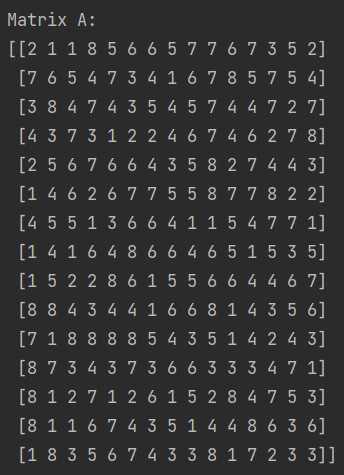
\includegraphics[width=0.6\textwidth]{matrix_A_3.jpg}
  \caption{Macierz gęsta A}
\end{figure}
\newpage

Losowanie wektora b prawej strony z wartościami losowymi.

\begin{figure}[h]
  \centering
  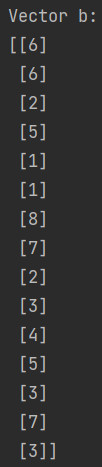
\includegraphics[width=0.1\textwidth]{vector_B_3.jpg}
  \caption{Wektor prawej strony b}
\end{figure}

Wyznaczenie macierzy L moim programem.

\begin{figure}[h]
  \centering
  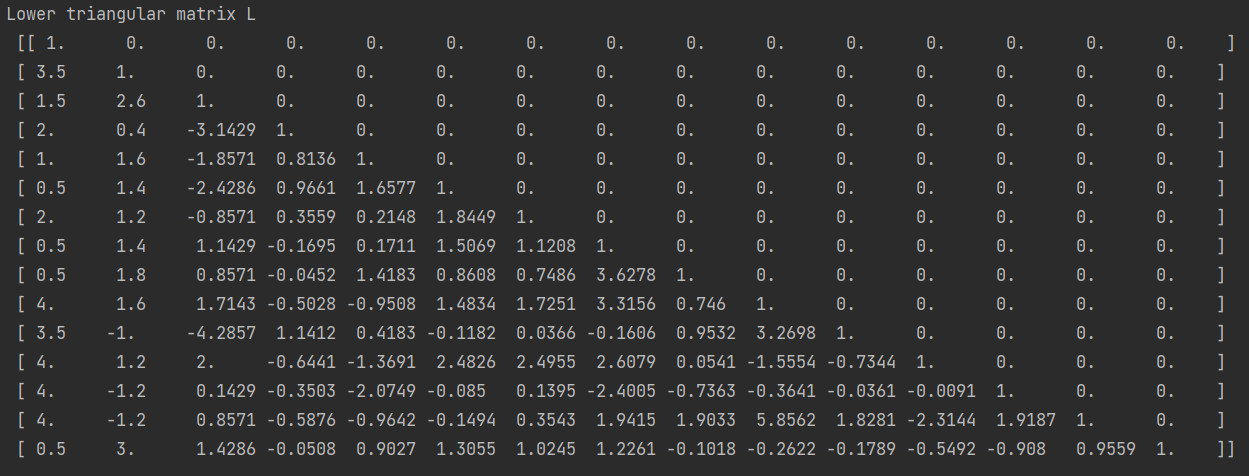
\includegraphics[width=0.9\textwidth]{L_1.jpg}
  \caption{Wyznaczona macierz L}
\end{figure}

Wyznaczenie macierzy U moim programem.

\begin{figure}[h]
  \centering
  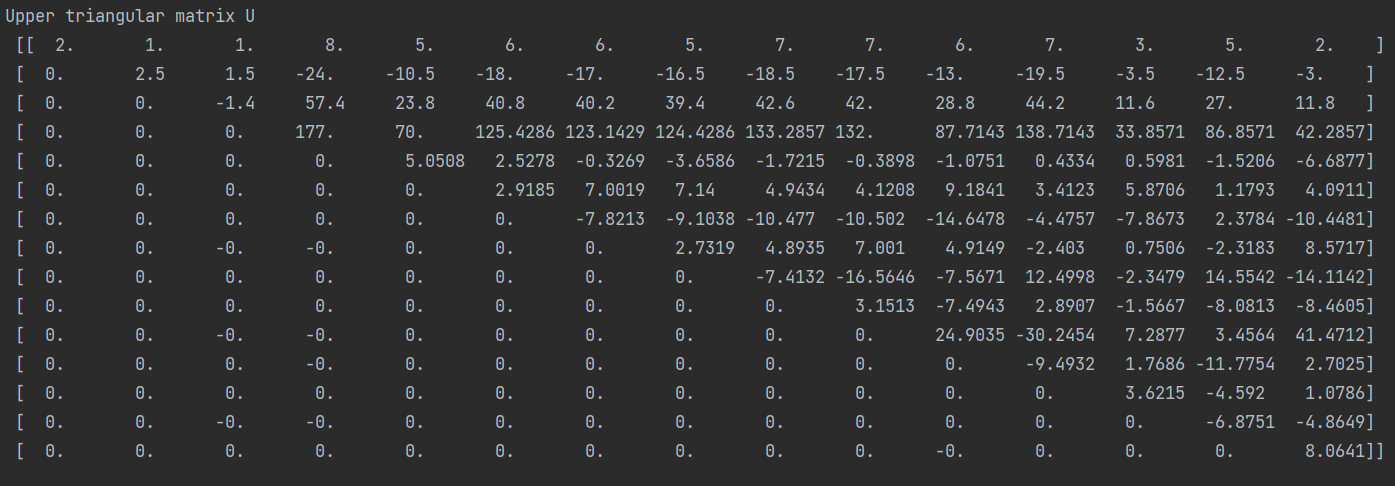
\includegraphics[width=0.9\textwidth]{U_1.jpg}
  \caption{Wyznaczona macierz U}
\end{figure}
\newpage

Wyznaczenie macierzy L, U i P programem MATLAB.

\begin{figure}[h]
  \centering
  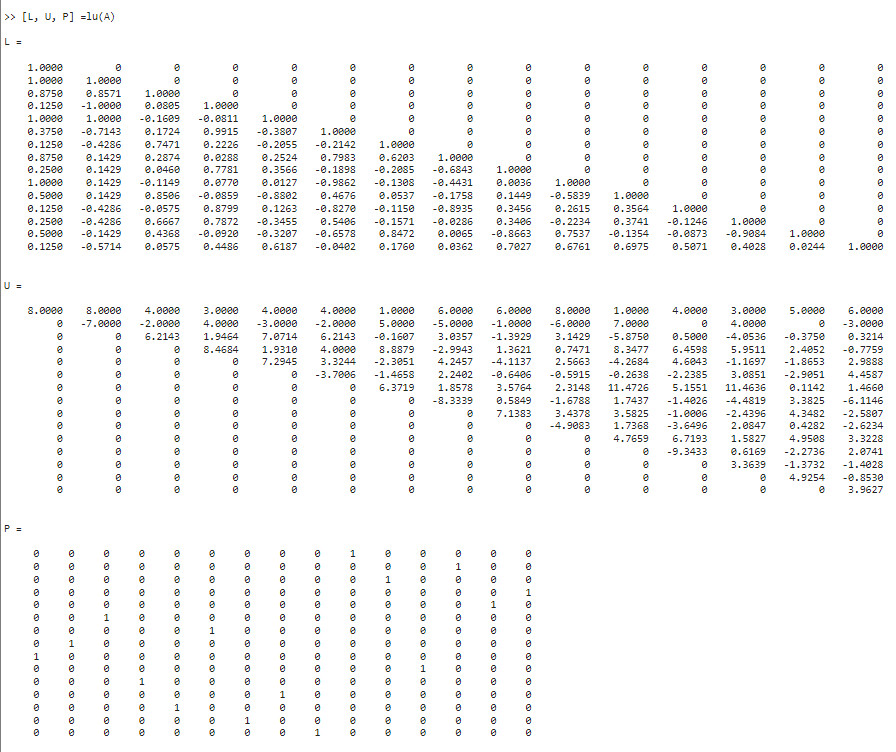
\includegraphics[width=0.9\textwidth]{L_U_P_1.jpg}
  \caption{Wyznaczone macierze L, U i P programem MATLAB}
\end{figure}
\newpage

Porównanie otrzymanych macierzy L i U mojego programu i MATLAB.

\begin{figure}[h]
  \centering
  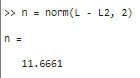
\includegraphics[width=0.2\textwidth]{L1_L2_comparison_1.jpg}
  \caption{Wynik norm(L1 - L2, 2) w MATLAB}
\end{figure}
\newpage

\begin{figure}[h]
  \centering
  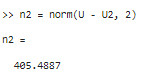
\includegraphics[width=0.2\textwidth]{U1_L2_comparison_1.jpg}
  \caption{Wynik norm(U1 - U2, 2) w MATLAB}
\end{figure}

Porównywane są tylko macierze L i U, ponieważ w części prezentacji o tej wersji algorytmu tylko te macierze były prezentowane.

Norma macierzowa 2-norm (lub norma spektralna) macierzy jest największą wartością osobliwą (wartością własną) macierzy. Wartość 11.6661 oznacza, że odchylenie (różnica) między macierzami L i L2 jest dość znaczące.

Wartość 405.4887 oznacza, że odchylenie (różnica) między macierzami U i U2 jest znaczące, mierząc je w kontekście tej konkretnej normy. Im większa wartość, tym większa różnica między macierzami. Można zatem powiedzieć, że większe róznice występują w macierzach U niż L.

\section{Algorytm LU faktoryzacji z pivotingiem}

\subsection{Pseudokod}

\begin{algorithm}
    \caption{LU factorization with pivoting}
    \begin{algorithmic}[1]
    
    \State $P \gets \text{identity matrix of size } A.\text{shape}[0]$
    \State $L \gets \text{identity matrix of size } A.\text{shape}[0]$
    \State $U \gets \text{copy of matrix } A$
    
    \For{$i \gets 0$ \textbf{to} $A.\text{shape}[0] - 1$}
        \State $\text{max\_element\_row\_index} \gets \text{index of maximum element in } [i, A.\text{shape}[0]) \text{ using } |\text{U[k, i]}|$
        \If{$i \neq \text{max\_element\_row\_index}$}
            \State $\text{Swap rows } i \text{ and } \text{max\_element\_row\_index}$ in $P$
            \State $\text{Swap rows } i \text{ and } \text{max\_element\_row\_index}$ in the first $i$ columns of $L$
            \State $\text{Swap rows } i \text{ and } \text{max\_element\_row\_index}$ in $U$
        \EndIf
        \For{$j \gets i + 1$ \textbf{to} $A.\text{shape}[0] - 1$}
            \State $L[j, i] \gets U[j, i] / U[i, i]$
            \State $U[j, i:] \gets U[j, i:] - (U[j, i] / U[i, i]) \times U[i, i:]$
        \EndFor
    \EndFor
    
    \State \textbf{return} $L, U, P$
    \end{algorithmic}
\end{algorithm}

Działanie programu można wyjaśnić następująco:

\begin{enumerate}
    \item Definicja funkcji: \texttt{lu\_factorization\_with\_pivoting(A: np.ndarray) -> tuple}. Funkcja przyjmuje macierz numpy \texttt{A} i zwraca trójkę zawierającą macierze L, U i P.
    \item Inicjalizacja macierzy pomocniczych:
    \begin{itemize}
        \item \texttt{P = np.eye(A.shape[0])}: Inicjalizuje macierz permutacji jako jednostkową macierz o rozmiarze odpowiadającym liczbie wierszy macierzy A.
        \item \texttt{L = np.eye(A.shape[0])}: Inicjalizuje dolną trójkątną macierz L jako jednostkową macierz o rozmiarze odpowiadającym liczbie wierszy macierzy A.
        \item \texttt{U = A.copy()}: Tworzy kopię macierzy A, która będzie górnotrójkątną macierzą U.
    \end{itemize}
    \item Pętla główna:
    \begin{itemize}
        \item Iteruje przez wiersze macierzy A używając zmiennej \texttt{i} w zakresie od 0 do liczby wierszy minus 1.
        \item Znajduje wiersz z maksymalną wartością bezwzględną w kolumnie \texttt{i} od \texttt{i} do ostatniego wiersza.
        \item Jeśli wiersz z maksymalną wartością bezwzględną nie jest aktualnie badanym wierszem \texttt{i}, dokonuje zamiany wierszy w macierzach P, L i U.
        \item Wewnętrzna pętla:
        \begin{itemize}
            \item Iteruje przez wiersze poniżej \texttt{i} (oznaczane przez \texttt{j} od \texttt{i+1} do końca).
            \item Oblicza wartości współczynników do aktualizacji macierzy L i U.
            \item Aktualizuje wartości w macierzy L i U.
        \end{itemize}
    \end{itemize}
    \item Zwrócenie wyników:
    \begin{itemize}
        \item Zwraca trójkę zawierającą macierze L, U i P.
    \end{itemize}
\end{enumerate}

\subsection{Kod algorytmu w języku Python}

\begin{figure}[h]
  \centering
  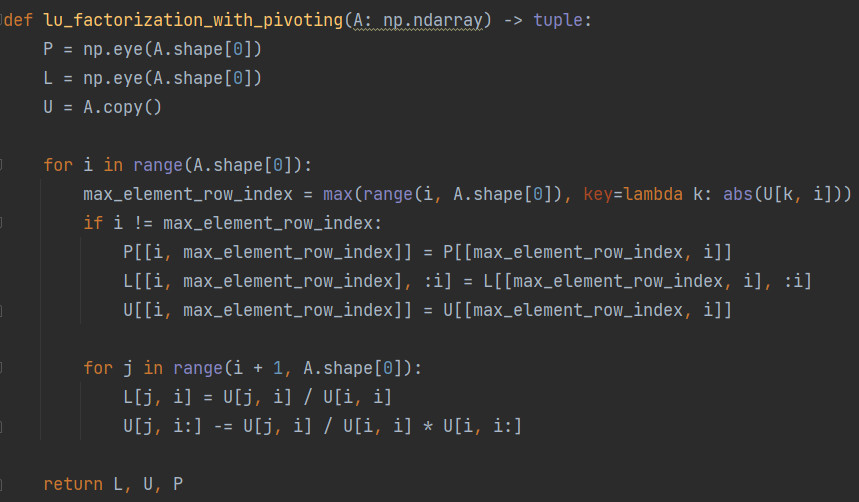
\includegraphics[width=0.9\textwidth]{lu_factoriaztion_with_pivoting.jpg}
  \caption{Kod algorytmu LU faktoryzacji z pivotingiem}
\end{figure}
\newpage

\subsection{Test dla macierzy gęstej o losowych wartościach (porównanie z MATLAB)}

Losowanie macierzy gęstej A z wartościami losowymi.

\begin{figure}[h]
  \centering
  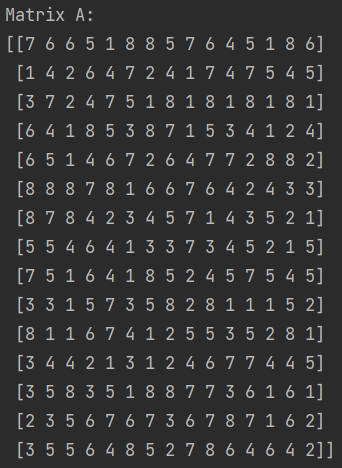
\includegraphics[width=0.6\textwidth]{matrix_A_4.jpg}
  \caption{Macierz gęsta A}
\end{figure}
\newpage

Wyznaczenie macierzy L moim programem.

\begin{figure}[h]
  \centering
  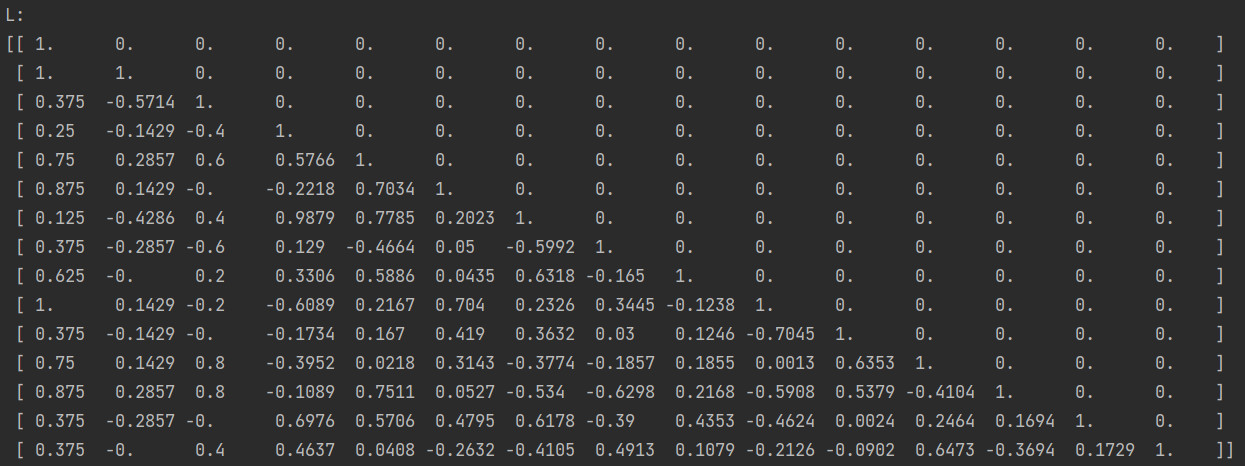
\includegraphics[width=0.9\textwidth]{L_2.jpg}
  \caption{Wyznaczona macierz L}
\end{figure}
\newpage

Wyznaczenie macierzy U moim programem.

\begin{figure}[h]
  \centering
  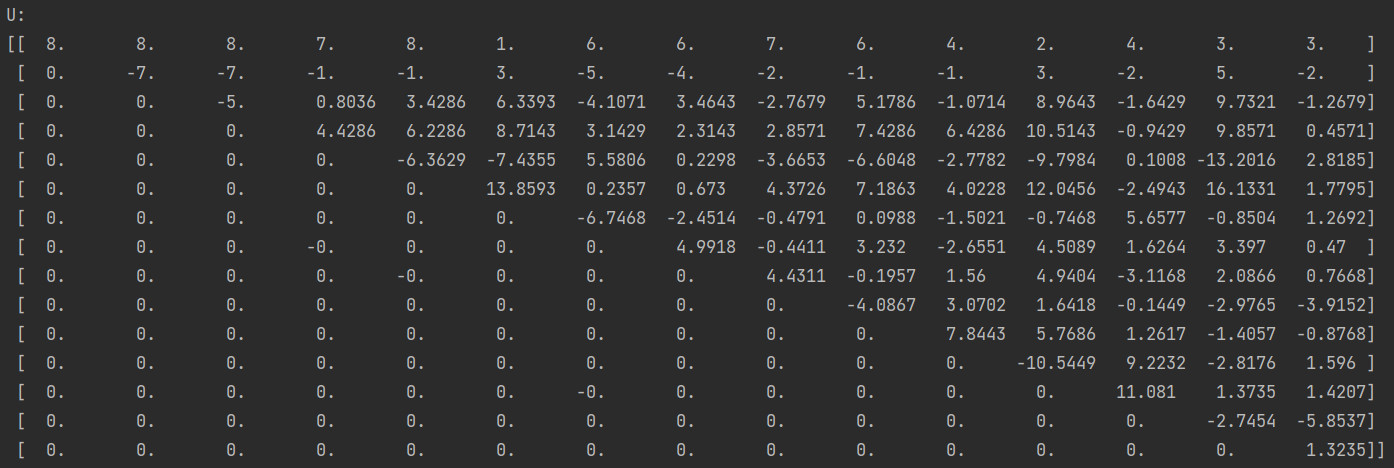
\includegraphics[width=0.9\textwidth]{U_2.jpg}
  \caption{Wyznaczona macierz U}
\end{figure}
\newpage

Wyznaczenie macierzy P moim programem.

\begin{figure}[h]
  \centering
  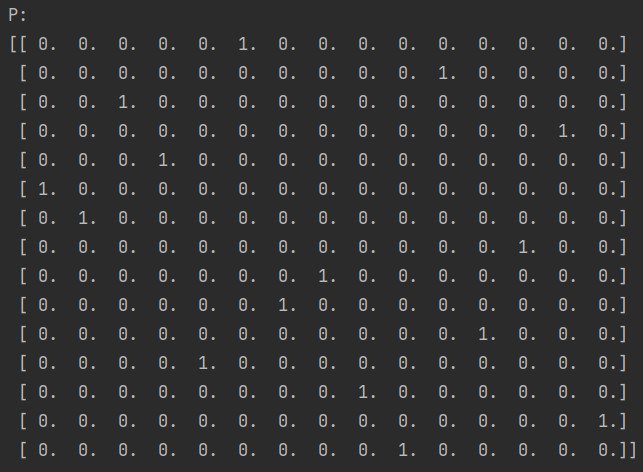
\includegraphics[width=0.9\textwidth]{P_2.jpg}
  \caption{Wyznaczona macierz P}
\end{figure}
\newpage

Wyznaczenie macierzy L, U i P programem MATLAB.

\begin{figure}[h]
  \centering
  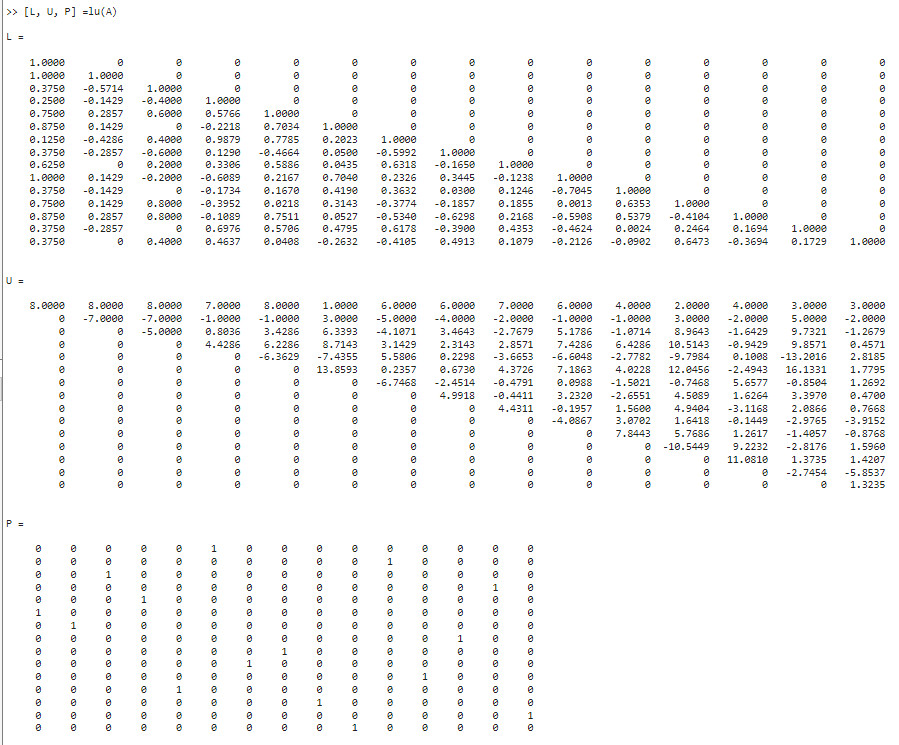
\includegraphics[width=0.9\textwidth]{L_U_P_2.jpg}
  \caption{Wyznaczone macierze L, U i P programem MATLAB}
\end{figure}
\newpage

Porównanie otrzymanych macierzy L, U i Pmojego programu oraz MATLAB.

\begin{figure}[h]
  \centering
  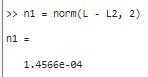
\includegraphics[width=0.2\textwidth]{L1_L2_comparison_2.jpg}
  \caption{Wynik norm(L1 - L2, 2) w MATLAB}
\end{figure}

\begin{figure}[h]
  \centering
  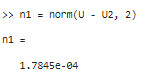
\includegraphics[width=0.2\textwidth]{U1_U2_comparison_2.jpg}
  \caption{Wynik norm(U1 - U2, 2) w MATLAB}
\end{figure}

\begin{figure}[h]
  \centering
  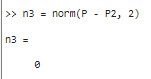
\includegraphics[width=0.2\textwidth]{P1_P2_comparison_2.jpg}
  \caption{Wynik norm(P1 - P2, 2) w MATLAB}
\end{figure}

Norma macierzowa 2-norm (lub norma spektralna) macierzy jest największą wartością osobliwą (wartością własną) macierzy. Wartość 1.4566e-04 oznacza, że odchylenie (różnica) między macierzami L i L2 jest bardzo mała.

Wartość 1.7845e-04 oznacza, że odchylenie (różnica) między macierzami U i U2 jest bardzo mała.

Wartość 0 oznacza, że nia ma odchylenia (różnica) między macierzami P i P2.

\section{Dlaczego niektóre wyniki się zgadzają z MATLABem a niektóre nie?}

Jedyne otrzymane wyniki, które zauważalnie nie zgadzały się z wynikami MATLAB były dla algorytmu LU faktoryzacji bez pivotingu. Uważam, że przyczyny wspominanych różnic wynikaja z:

 - mogą występować różnice w implementacji operacji arytmetycznych, co może prowadzić do różnic w precyzji obliczeń;

- mimo, że algorytmy są podobne, drobne różnice w implementacji mogą prowadzić do różnic w wynikach. To może wynikać z różnic w implementacji operacji arytmetycznych czy optymalizacji kodu;

- różnice w wynikach mogą się również pojawić ze względu na różnice w sposobie zaokrąglania liczb i obsługi punktów stałoprzecinkowych. W MATLAB zauważyłem, że liczby były zaokrąglane do 4 miejsc po przecinku, a w Python poza zaokrągleniem wyniku nie miało to miejsca,

- sposób wczytywania i przetwarzania danych może się różnić między Python a MATLAB, co może wpływać na wyniki.

\section{Czy da się wylosować taką macierz żeby wszystkie wyniki się zgadzały?}

Uważam, że przy stworzeniu odpowiednich warunków jest możliwe uzyskanie zgodnych wyników. Przykładowo można:

 - wygenerować macierz i wektor tak, aby spełniały określone warunki, które sprawią, że wyniki działania algorytmów będą takie same.

- z ustawić konkretne wartości macierzy i wektora prawych stron w taki sposób, aby były one identyczne dla obu algorytmów.

- wybrać proste dane testowe, dla których wyniki algorytmów są dobrze znane i można je łatwo zweryfikować.

\end{document}